\providecommand{\AppPlaceholder}[2]{%
    \fbox{
        \begin{minipage}[c][#1][c]{0.94\textwidth}
            \centering
            \textit{#2}
        \end{minipage}
    }
}

\begin{figure*}[t]
\centering
\vspace{-2mm}
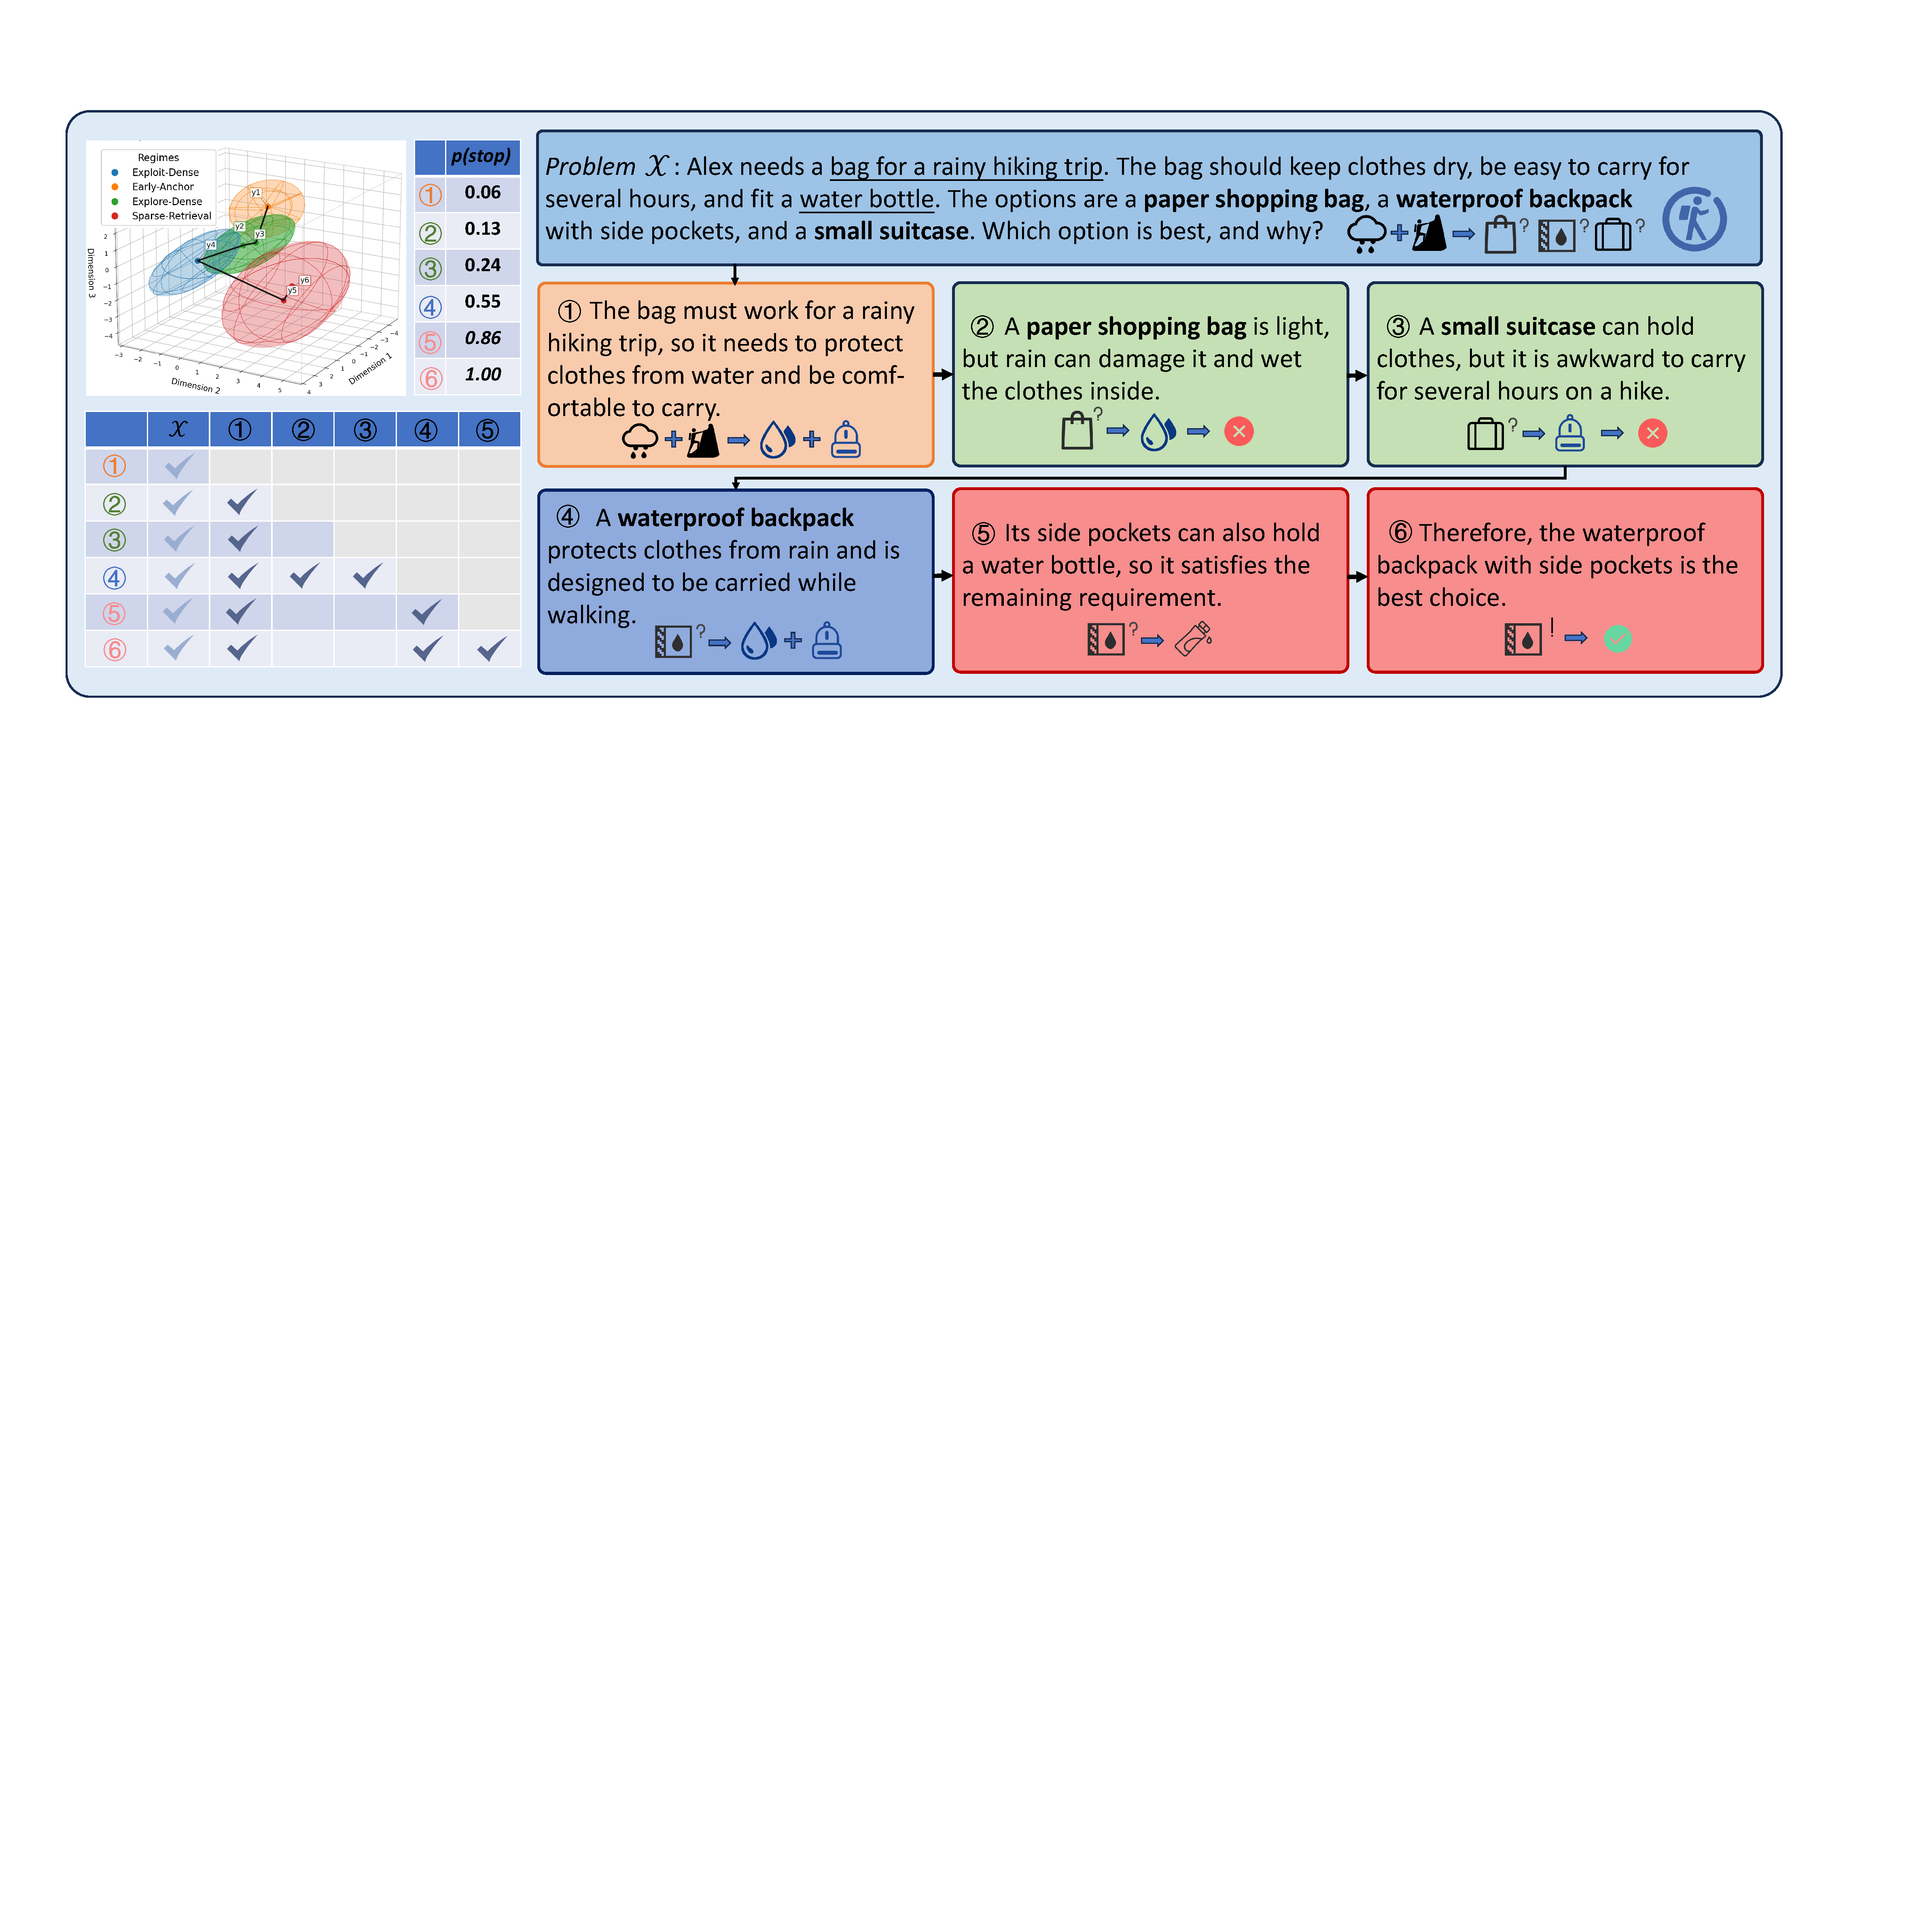
\includegraphics[width=0.98\textwidth]{figs/app_case.pdf}
\vspace{-2mm}
\caption{\textbf{A case study of SoT,} with more case studies in Appendix~\ref{app:case_studies}.}
\label{fig:app_case}
\vspace{-5mm}
\end{figure*}

    \vspace{-1mm}
    \section{Exploratory Extensions of State of Thought}
    \label{sec:explore}
    \vspace{-1mm}
    
    \subsection{SoT under Limitation}
    \label{sec:training_free_sot}
    \vspace{-0.5mm}
    \paragraph{Training-Free SoT.}
    We first ask \emph{whether SoT requires learned control at all}. We instantiate the evidence-organization operator \(\mathcal{S}\) and stopping operator \(\mathcal{T}\) without training, using fixed rules derived from the same dynamics-geometric state.
    Historical evidence is selected by state compatibility with the current reasoning regime, while stopping is triggered when the trajectory becomes sufficiently stable and low-uncertainty.
    This yields a fully training-free SoT controller that preserves the same closed-loop formulation while removing learned control entirely.

    \vspace{-0.5mm}
    \paragraph{SoT-Embed under Limited Access.}
    We next ask \emph{whether SoT depends on privileged access to internal information transfer}.
    We embed the model's multi-step segmented output with a fixed encoder and feed the embedding trajectory into the control loop in place of the internal state.
    This tests whether endogenous reasoning control remains viable when the interface is weakened to text.
   
    SoT-Training-free evaluates whether the benefits of SoT come solely from the learned controller, while SoT-Embed tests whether it relies on white-box access. 
    Table~\ref{tab:boundary_sot} summarizes that both variants maintain competitive performance, with macro-averaged accuracy lower relative to full SoT by approximately \(16.4\%\) for SoT-Training-free and \(16.0\%\) for SoT-Embed. In comparison, the Top-3 baseline methods show an average accuracy of \(47.6\%\) on those cells, with SoT variants achieving comparable or slightly better results in many tasks. These results suggest that SoT's core advantage lies in the principle of state-conditioned evidence organization, not in a specific implementation. Despite these reductions relative to full SoT, both variants remain highly competitive, often outperforming the Top-3 baselines on this Llama table. For further details, see Appendix~\ref{app:limitations_sot}.

    \begin{table*}[t]
    \centering
    \vspace{-1mm}
    \caption{\textbf{Boundary studies of SoT on Llama-3.1-8B,} with other models provided in Table~\ref{tab:app_boundary_qwen}, ~\ref{tab:app_boundary_mixtral}.}
    \vspace{-2mm}
    \label{tab:boundary_sot}
    \footnotesize
    \setlength{\tabcolsep}{5pt}% 正文 boundary：列间略疏，数值不挤；与附录同行距
    \renewcommand{\arraystretch}{1.05}% 行距略抬高，缓和贴线；色块仍需 rule sep 为 0
    \begingroup
    \setlength{\aboverulesep}{0pt}%
    \setlength{\belowrulesep}{0pt}%
    \setlength{\extrarowheight}{0.95pt}%
    \begin{tabular}{l!{\vrule width 0.4pt}*{4}{c}!{\vrule width 1pt}*{6}{c}}
    \toprule
    & \multicolumn{4}{>{\cellcolor[HTML]{E3F2FD}}c!{\vrule width 1pt}}{\textbf{Quantitative Reasoning}} & \multicolumn{6}{>{\cellcolor[HTML]{E3F2FD}}c}{\textbf{Symbolic and Code}} \\
    \cmidrule(lr){2-5}\cmidrule(lr){6-11}
    & GSM8K & MATH & DROP & avg. & FOLIO & PW & BBH-T & HE & MBPP & avg. \\
    \midrule
    Top-3 Baseline avg.        & 82.9 & 61.5 & 16.2 & 53.5 & 40.6 & 37.6 & 60.0 & 30.0 & 52.0 & 44.0 \\
    SoT-Training-free          & 81.8 & 60.5 & 34.6 & 59.0 & 34.6 & 30.2 & 77.0 & 53.0 & 50.8 & 49.1 \\
    SoT-Embedding             & 82.8 & 61.8 & 32.3 & 59.0 & 33.8 & 30.5 & 74.0 & 57.9 & 52.8 & 49.8 \\
    \midrule
    \end{tabular}
    \par\addvspace{0.35ex}%
    \begin{tabular}{l!{\vrule width 0.4pt}*{6}{c}!{\vrule width 1pt}*{4}{c}}
    & \multicolumn{6}{>{\cellcolor[HTML]{E3F2FD}}c!{\vrule width 1pt}}{\textbf{General Understanding}} & \multicolumn{4}{>{\cellcolor[HTML]{E3F2FD}}c}{\textbf{Long-Context Reasoning}} \\
    \cmidrule(lr){2-7}\cmidrule(lr){8-11}
    & CSQA & StrQA & BoolQ & MMLU & RACE & avg. & HQA & NarQA & LB & avg. \\
    \midrule
    Top-3 Baseline avg.         & 50.3 & 68.6 & 78.9 & 53.3 & 56.5 & 61.5 & 15.6 & 25.4 & 31.7 & 24.2 \\
    SoT-Training-free          & 37.5 & 55.2 & 70.0 & 45.4 & 53.0 & 52.0 & 21.8 & 34.2 & 27.3 & 27.8 \\
    SoT-Embedding             & 37.5 & 56.8 & 71.2 & 41.8 & 52.0 & 51.9 & 28.5 & 30.3 & 27.1 & 28.6 \\
    \bottomrule
    \end{tabular}%
    \endgroup
    \vspace{-5mm}
    \end{table*}

    \vspace{-2mm}
    \subsection{SoT as a Trajectory-Level Judge}
    \label{sec:judge}
    \vspace{-3mm}
    
    % twocolumn 下 wraptable 常失效；用并排 minipage（同栏内）可与正文并排，且不依赖 wrapfig。
    \noindent
    \begin{minipage}[t]{0.52\columnwidth}%
        \vspace{0pt}%
        We further study \emph{whether information visible only in the completed reasoning trace can support black-box quality assessment}, without online control or access to hidden states.
        Given sentence-segmented model outputs, we map each step to a standard sentence embedding and summarize the resulting sequence using compact trajectory statistics, with details in Appendix~\ref{app:sot_judge}.
        A small trainable predictor (\textsc{SoT-Judge}) then estimates whether the final answer matches reference correctness.
        The goal is a clean trajectory-only readout of reasoning health, parallel in spirit to SoT's use of trajectory organization, but reduced to post-hoc inputs that any API model exposes. We evaluate three closed or API-accessed models: GPT-5.4 \citep{openai2025gpt54}, Claude Opus 4.7 \citep{anthropic2026claudeopus47}, and Qwen-Max \citep{alibaba2026qwenmax}.
    \end{minipage}%
    \hfill
    \begin{minipage}[t]{0.45\columnwidth}%
        \vspace{0pt}%
        \centering
        \captionsetup{font=footnotesize,position=top,aboveskip=2pt,belowskip=3pt,skip=0pt}%
        \captionof{table}{\textbf{Black-box judging with trajectory-based SoT} (agreement with reference correctness).\label{tab:blackbox_judge}}%
        \vspace{0mm}%
        \footnotesize
        \setlength{\tabcolsep}{2.25pt}%
        \begingroup\setlength{\aboverulesep}{0pt}\setlength{\belowrulesep}{0pt}%
        \setlength{\extrarowheight}{0.75pt}%
        \renewcommand{\arraystretch}{1.1}%
        \begin{adjustbox}{max width=\linewidth,center}%
        \begin{tabular}{@{}l@{ }lcccc>{\columncolor[HTML]{EAECEF}\centering\arraybackslash}c@{}}%
        \toprule
        \textbf{Model} & \textbf{Method}
        & \makecell{\textbf{QR}}
        & \makecell{\textbf{GU}}
        & \makecell{\textbf{S\&C}}
        & \makecell{\textbf{LCR}}
        & \textbf{avg.} \\
        \midrule
        \multirow{4}{*}{GPT-5.4}
        & Self-Consistency & 65.6 & 81.7 & \underline{77.8} & 12.3 & 59.3 \\
        & Self-Verification & 65.6 & 80.8 & 77.4 & 11.9 & 58.9 \\
        & LLM-as-a-Judge & 65.7 & \underline{82.2} & 77.7 & 12.1 & 59.4 \\
        & \textbf{SoT-Judge} & \textbf{\underline{87.2}} & \textbf{80.4} & \textbf{77.2} & \textbf{\underline{84.0}} & \textbf{\underline{82.2}} \\
        \midrule
        \multirow{4}{*}{\makecell[c]{Claude\\Opus 4.7}}
        & Self-Consistency & 63.8 & \underline{83.5} & 76.2 & 5.9 & 57.3 \\
        & Self-Verification & 66.9 & 60.8 & \underline{82.3} & 11.5 & 55.4 \\
        & LLM-as-a-Judge & 64.0 & \underline{83.5} & 76.6 & 6.0 & 57.5 \\
        & \textbf{SoT-Judge} & \textbf{\underline{89.0}} & \textbf{82.7} & \textbf{77.0} & \textbf{\underline{95.7}} & \textbf{\underline{86.1}} \\
        \midrule
        \multirow{4}{*}{Qwen-Max}
        & Self-Consistency & 65.0 & 83.5 & \underline{80.5} & 10.6 & 59.9 \\
        & Self-Verification & 32.7 & \underline{86.2} & 78.6 & 6.6 & 51.0 \\
        & LLM-as-a-Judge & 66.7 & 84.2 & 80.4 & 11.1 & 60.6 \\
        & \textbf{SoT-Judge} & \textbf{\underline{88.5}} & \textbf{84.8} & \textbf{75.5} & \textbf{\underline{87.1}} & \textbf{\underline{84.0}} \\
        \bottomrule
        \end{tabular}%
        \end{adjustbox}%
        \endgroup
        \vspace{-6mm}% 收窄表下空白（双栏并排时常留下大块留白）
    \end{minipage}

    \par\vspace{-1mm}%
    \noindent
    
    We compare against three representative black-box judging strategies, including Self-Consistency~\citep{wang2023selfconsistency}, Self-Verification~\citep{weng2023large}, and LLM-as-a-Judge~\citep{zheng2023judging}, covering sample-based agreement, self-verification, and external judging. By contrast, \textsc{SoT-Judge} predicts correctness only from the embedded sentence trajectory, without extra rollouts, self-critique passes, or stronger external judge calls. Table~\ref{tab:blackbox_judge}, with breakdown in Table~\ref{tab:app_judge_breakdown}, shows that \textsc{SoT-Judge} improves the average agreement over the strongest baseline by \(+22.8\), \(+28.6\), and \(+23.4\) points on GPT-5.4, Claude Opus 4.7, and Qwen-Max, respectively. The gain is not uniform across domains: on GU and S\&C, trajectory-only judging is mostly comparable to standard judges, while the largest improvements come from QR and especially LCR, where agreement of black-box baselines drops to \(5.9\)--\(12.3\%\) but \textsc{SoT-Judge} remains at \(84.0\)--\(95.7\%\). This suggests that trajectory structure provides a useful correctness signal, especially when black-box judging becomes unreliable under sparse or long-range evidence.